\documentclass[A4paper, punct,space,nospace, fancyhdr, fntef,UTF8]{ctexart}

\usepackage{itils}%在这里放置需要的宏包,并设置部分所需内容
\usepackage[toc,page]{appendix}
\renewcommand\appendixname{Appendix}
\renewcommand\appendixtocname{Appendix}
\renewcommand\appendixpagename{Appendix}
\begin{document}
	\pagestyle{empty}%不要页眉页脚
	%封面与诚信声明
	


\begin{figure}[htbp]
	\begin{center}
		
\includegraphics[width=4.7in]{logo}%在sty文件里已经设置了图片文件夹路径了
	\end{center}
\end{figure}
\vskip 1cm
\centerline{
	\songti\zihao{2}{2020年“深圳杯”数学建模挑战赛}%反斜杠=空一格
}
\vskip 2cm
\centerline{
	\songti\zihao{2}{近地飞行器视觉稠密建图(Dense-Mapping)系统}%反斜杠=空一格
}
\vskip 1.5cm


\centerline{\songti\zihao{4}{版本编号:20200628v2}}
\vskip 1cm
\centerline{\songti\zihao{4}{2020. 08. 10}}
%表格
\begin{comment}
	\begin{flushleft}
		\centering
			\begin{tabular}{|c|l|l|c|l|l|}
				
				\hline
				\multicolumn{6}{|c|}{
					\multirow{2}{*}{
						\heiti{队伍名称:}
						\kaishu{\quad\textbf{兴奋剂}\hspace{0.5cm}}
					}
				}\\
				\multicolumn{6}{|c|}{}\\
				
				\hline
				\multicolumn{3}{|c|}{
					\multirow{2}{*}{
						\heiti{王祥通}
						%\kaishu{\quad\textbf{□口试\ □笔试\ □撰写论文 }\hspace{0.5cm}}
					}
				} & \multicolumn{3}{c|}{
					\multirow{2}{*}{
						\heiti{四川大学空天科学与工程学院}
						%\kaishu\underline{\quad\textbf{}\hspace{1cm}}
					}
				} \\
				
				\multicolumn{3}{|c|}{}& \multicolumn{3}{c|}{} 
				
				\\ \hline
				\multicolumn{3}{|c|}{
					\multirow{2}{*}{
						\heiti{None}
					%	\kaishu\underline{\quad\textbf{周广武 }\hspace{0.5cm}}
					}
				} & \multicolumn{3}{c|}{
					\multirow{2}{*}{
						\heiti{None}
						%\kaishu\underline{\quad\textbf{ }\hspace{1cm}}
					}
				} \\
				\multicolumn{3}{|c|}{}& \multicolumn{3}{c|}{}
				
				\\ \hline
			\end{tabular}
			
		\end{flushleft}
\end{comment}


\vskip 1cm
\centerline{\songti\zihao{4}{参赛组别: 创意应用}}

%\vskip 4cm
%\centerline{\heiti\zihao{2}{四\ 川\ 大\ 学\ 研\ 究\ 生\ 院\ 制 }}%反斜杠=空一格
%\vspace{10bp}
%\centerline{\zihao{3}{2019 年 \  1 月\ }}


	
	\zihao{-4}
	\tableofcontents%生成目录
	\thispagestyle{empty}%页脚不要页码
	%“目录”两个字的样式与section的样式一致,默认居中,故将设置section标题居左放置在生成目录后
	\CTEXsetup[format={\large\bfseries}]{section}  %section标题居左
	
	
	
	%\newpage
\begin{table}
	\begin{center}
		\caption{变更记录}
		\begin{tabular}{l|ccccc}
			\toprule[2pt] 
			序号   &  更改原因 & 版本&作者&更改日期&备注 \\ \hline
			00& 初始化&20200606v1&王祥通&20200606& none\\
			01&日常更新&20200628v2&王祥通&20200628&补充内容\\
			02&日常更新&20200801v3&杨帆,朱璇&20200801&补充背景以及应用部分内容\\
			03&日常更新&20200805v4&毛明洋&20200805&补充相关实验\\

			\toprule[2pt] 
		\end{tabular}
		
		\label{tab:log}
		\vspace{-0.4cm}
	\end{center}
\end{table}
	
	
	
	
	
	%%%%正文开始,页脚有页码
	\cfoot{\zihao{-5}第 \ \thepage \ 页 \ 共 \ \pageref{lastpage} 页}
	
	%lastpage为末页标签要在最后一页加上代码 \label{lastpage}%显示总页数
	
	
	
	
	%正文
	\zihao{5} 
	\pagenumbering{arabic}%页码使用阿拉伯数字
	\setcounter{page}{0}  %重新设置页码计数
	\pagestyle{fancy}

	%章节内容
	\newpage


\centerline{\fangsong\bf\zihao{-2}{无线可充电传感器网络充电路线规划}}
\addcontentsline{toc}{section}{摘要(关键词)}%加入目录


\vskip 1cm


\vskip 10bp

{
	\kaishu	
	\hspace{5bp}{\zihao{-4}\textbf{【摘要】}} 
	本文涉及的问题为旅行商问题以及优化问题, 我们主要通过人工神经网络方法建立模型, 求解问题.
	
	针对问题1, 我们引入自组织映射网络(Self-Organizing Map,SOM), 通过竞争合作学习的方法, 求出最优路径:

	$p_{0}\rightarrow p_2\rightarrow p_1\rightarrow p_9\rightarrow p_7\rightarrow p_6\rightarrow p_{14}\rightarrow p_{11}\rightarrow p_{8}\rightarrow  p_{12}\rightarrow  p_{15}\rightarrow  p_{27}\rightarrow  p_{16}\rightarrow  p_{13}\rightarrow  p_{10}\rightarrow p_{5}\rightarrow p_{3}\rightarrow p_{4}\rightarrow p_{22}\rightarrow  p_{28}\rightarrow p_{24}\rightarrow p_{23}\rightarrow p_{21}\rightarrow p_{29}\rightarrow p_{26}\rightarrow p_{25}\rightarrow p_{18}\rightarrow p_{19}\rightarrow p_{20}\rightarrow p_{17}$
	路径长度$l= 0.1143807$,换算成SI单位制后,$l=11.43807 km$.
	
	针对问题2, 本文建立优化模型, 通过最小化每个结点的充电时间建模求解而得到电池电量的允许最低值的解析解.
	
	针对问题3, 我们将自组织映射网络方法进一步推广, 构建四个神经元环, 将问题自然的过度到多旅行商问题(Multiple Traveling Salesmen Problem, mTSP), 并求解出四条路径为:
	\begin{eqnarray}
		\nonumber
	G_A = p_0 \rightarrow p_3 \rightarrow p_{28} \rightarrow p_{24} \rightarrow p_{23} \rightarrow p_{22} \rightarrow p_{4}, \text{路径长度} l_A = 0.031713;\\ 
	\nonumber
	G_B = p_0  \rightarrow p_{17} \rightarrow p_{19} \rightarrow p_{29} \rightarrow p_{26} \rightarrow p_{25} \rightarrow p_{18} \rightarrow p_{20}, \text{路径长度}l_B = 0.035541;\\
	\nonumber
	G_C = p_{0} \rightarrow p_{1} \rightarrow  p_{9} \rightarrow  p_{7} \rightarrow  p_{6} \rightarrow  p_{14} \rightarrow  p_{11} \rightarrow   p_{7} \rightarrow  p_{2} , \text{路径长度} l_C = 0.0408157;\\
	\nonumber
	G_D = p_{0} \rightarrow  p_{10} \rightarrow  p_{12} \rightarrow  p_{15} \rightarrow  p_{27} \rightarrow  p_{16} \rightarrow  p_{13} \rightarrow  p_{5} , \text{路径长度} l_D = 0.028521; 
	\end{eqnarray}

	路程总计$l = l_A +l_B+l_C+l_D = 0.13659$,换算成SI单位制 $l=13.659 km$. 详细见拓扑图\ref{fig:mtsp-solution}. 此外,对多路径下的电池容量问题, 我们借助问题2的模型, 给出了四条子路径下各自电池容量最低值的解析解, 其最大值则为整个系统可允许的电池最低容量.

	最后, 为了对SOM网络性能更进一步说明, 我们将SOM模型与其变种和常见的进化算法在TSP问题公开数据集上进行了对比, 结果表明在点数较少时($N \leq 100$)时, SOM类算法优势并不明显, 当点数较多时($N \geq 100)$, SOM类的方法精度与效率明显优于其他.
	 本文代码全部开源, 详情可见支撑材料或\url{https://github.com/xdr940/M2CT2020}

	
	\vskip 10bp
	
	\hspace{5bp} {\zihao{-4}\textbf{【 关键词】}} 
	旅行商问题(TSP), 多旅行商问题(mTSP), 自组织映射网络(SOM) 
}
	\section{问题重述与分析}
	\subsection{问题重述}

	随着物联网的快速发展,无线传感器网络WSN(Wireless Sensor Network)在生活中的应用也越来越广泛. 无线传感器网络中包括若干传感器(Sensors)以及一个数据中心(Data Center)。传感器从环境中收集信息后每隔一段时间将收集到的信息发送到数据中心. 数据中心对数据进行分析并回传控制信息.
	影响WSN生命周期最重要的一个因素是能量. 想要让WSN能够持续不断地运转, 就必须持续为WSN提供能量. 提供能量的方式之一是能量收集(Energy Harvesting), 通过利用太阳能或风能等环境能源让传感器自行从环境中汲取能量以维持其运作, 然而这种方式提供的能量不但不稳定,而且太过于依赖环境, 一旦环境达不到条件,WSN无法从环境中汲取能量自然也就无法运转.
	
	提供能量的另外一种方式是电池供电, 并利用移动充电器定期为传感器的电池补充能量, 从而源源不断地为WSN提供稳定的能量使其正常运转. 通过这种方式供电的网络也被称为无线可充电传感器网络WRSN(wireless Rechargeable Sensor Network)

	考虑使用第二种方式供电, 为了让WRSN正常运转,移动充电器需要定期为传感器进行充电以避免其电量低于阈值. 移动充电器从数据中心出发, 以固定的速度依次经过每个传感器, 在每个传感器处停留一段时间并以固定的充电速率为传感器充电, 直到为所有传感器充电完成之后返回数据中心. 每个传感器都有\textbf{特定}的能量消耗速率, 以及\textbf{固定}的电池容量. 移动充电器的能量消耗主要有两个方面:一是为传感器节点充电所导致的正常的能量消耗; 另外一方面则是移动充电器在去为传感器充电的路上的能量消耗.

	\begin{itemize}
		\item 问题一: 给定数据中心结点和传感器的位置信息, 通过一辆车从数据中心结点出发, 依次经过传感器结点, 并使得路程消耗最低.
		\item 问题二:给定每个结点的位置$x_i,y_i$和能量消耗率$w$, 以及传感器电池允许的最低电量$f(mA/h)$,通过一辆车, 并沿着问题一的结果路线, 求出个传感器的电池的容量应至少是多大才能保证整个系统一直正常运行(即系统中每个传感器的电量都不会低于$f(mA/h)$.
		\item 问题三:给定每个几点的位置和能量消耗, 以及传感器允许最低点亮, 移动充电车的速度$v(m/s)$,移动充电车的充电速率$r(mA)$, 通过四辆车, 如何规划线路, 使得充电车的路上总能量消耗最小?每个传感器的电池容量应该是多大才能保证整个系统一直运行.
	\end{itemize}
	
	
	




	%\begin{table}[h]
	\begin{center}
		\caption{队员分工}
		\begin{tabular}{l|cc}
			\toprule[2pt] 
			   &  符号 & 意义 \\ \hline
			01& $i$& 结点标号\\
			03& $(x_i,~y_i)$&结点i的坐标\\
			04& $w_i$&结点i消耗率\\
			04& $w_i$&结点i电量消耗速率\\
			04& $f$&结点电池电量底线\\
			04& $m$&结点电池电量\\

			02& $k$&充电车标号\\
			02& $v$&充电车速度\\
			02& $r$&充电车充电速率\\
			
			04& $l_{i,j}$&两个结点的距离\\
			\toprule[2pt] 
		\end{tabular}
		
		\label{tab:distribution}
		\vspace{-0.4cm}
	\end{center}
\end{table}



	\subsection{问题分析}
		
		问题一中, 给定信息包括传感器结点坐标以及出发点数据中心的坐标, 在题干中并没有各个传感器结点对充电车的序列要求, 所以可以抽象为一个典型的旅行商(TSP)问题而非更一般的的车辆路径问题(VRP).

		问题二中, 在已知路径总距离的情况下, 充电车运行一圈时间应该是固定的, 若要使得电池容量最小, 则需要最大电量结点最小. 另外, 在系统处于临界时, 冲电车对每个结点充电时刻恰好为该结点电量耗光时刻, 即放电时间小或等于等待时间, 通过以上联系, 可以建立优化模型求解任意结点的充电最小时间.

		问题三中, 给定四辆充电车, 这里有两个目标, 一个是使得传感器电池容量最小, 另一个是让充电车上的能量损耗最小, 所以各个车辆在找到各自回路的同时应该尽量保证路过的结点数量相似. 该问题可抽象为多重旅行商问题(mTSP), 其中履行商个数对应着充电车数量即$m=4$,仓库点个数$depot= 1$.
		






		\subsection{模型假设}
		%为了对问题分析更加有方向性, 忽略本文建立模型假设如下
		\begin{itemize}
			\item 所以结点电池规格完全一样.
			\item $r$为净充电速率, 不考虑掉电影响.
			\item 传感器结点张成的为平面坐标系, 经纬度换算统一为$0.00001\deg/1m$
		\end{itemize}
	
\section{模型准备}
\label{sec:preliminary}
本节简要介绍自组织映射神经网络(SOM)以及相关知识.

\subsection{模型符号说明}

\begin{table}[h]
	\begin{center}
		\caption{SOM模型相关符号说明}
		\begin{tabular}{l|c}
			\toprule[2pt] 
			    符号 & 意义 \\ \hline
			 $X_i$& 样本结点\\
       $W_j$&神经元结点\\
       $n$&迭代步数\\
       $\sigma$&邻域半径\\


			\toprule[2pt] 
		\end{tabular}
		
		\label{tab:distribution}
		\vspace{-0.4cm}
	\end{center}
\end{table}


\subsection{自组织映射神经网络}
\label{sec:som}
自组织映射神经网络(Self-Organizing Map, SOM)或自组织特征映射(Self-Organizing Features Map, SOFM)是一种无监督的人工神经网络, 于1982年被Kohonen提出\cite{som}. 不同于一般神经网络基于损失函数的反向传递误差来训练, 它运用竞争学习(competitive learning)策略, 依靠神经元之间互相竞争逐步优化网络,且使用近邻关系函数(neighborhood function)来维持输入空间的拓扑结构.

\begin{figure}[h]
    \begin{center}
        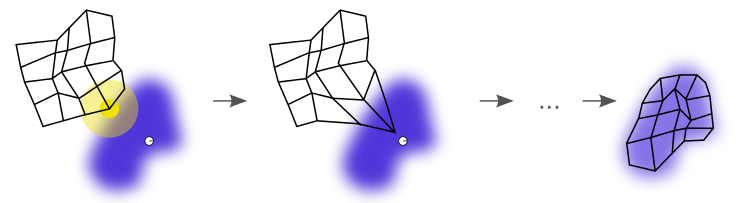
\includegraphics[width=0.6\linewidth]{fig/som1}
    \end{center}
    \caption{\textbf{SOM训练过程示意图.} 图来自wiki}
        \label{fig:plan}
  \end{figure}

\subsection{网络结构}

自组织神经网络本质上是一个两层的神经网络,包含输入层和输出层(竞争层). 输入层模拟感知外界输入信息的视网膜,输出层模拟做出响应的大脑皮层. 输入层的神经元数量由输入的维度决定, SOM网络结构的区别主要在竞争层: 可以有1维、2维(最常见的)

自组织映射的可见部分是映射空间(竞争层), 它由称为节点或神经元的单元组成。预先定义了映射空间,通常将其定义为有限的二维区域,其中节点以规则的六边形或矩形网格或排列, 见图\ref{fig:som2} 
\begin{figure}[h]
    \begin{center}
        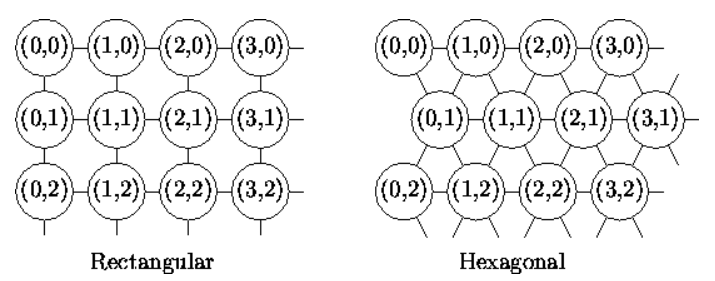
\includegraphics[width=0.6\linewidth]{fig/som2}
    \end{center}
    \caption{\textbf{SOM竞争层排列方式.} }
        \label{fig:som2}
  \end{figure}

在映射空间中, 每个神经元节点都与一个"权重"向量相关联, 该向量表征的是输入空间中的位置. 也就是说,神经元在数据结构上具有与每个输入向量(样本)相同的尺寸, 维度相同. 在映射空间中的节点保持固定的同时,训练包括将权重向量移向输入数据(减少距离度量, 而不会破坏从映射空间的拓扑。因此,自组织映射描述了从高维输入空间到低维映射空间的映射.
训练后, 该映射可以通过找到权重向量与输入空间向量最近(最小距离度量)最近的节点来对输入空间中的向量进行分类.%这句不明白

数人工神经网络一样,SOM以两种模式运行: 训练和映射. "训练"使用输入示例(竞争过程,也称为矢量量化)构建地图, 而"映射"自动分类新的输入矢量.

\subsection{网络训练}

网络训练的过程, 就是将输出层结点尽可能的扩张到训练集空间的过程, 其可以分为以下几个步骤:

\begin{itemize}
    \item[\textbf{0}] 初始化: 将神经元的权重初始化为较小的随机值,或者从两个最大主成分 特征向量跨越的子空间中均匀采样\footnote{使用后一种替代方法,学习速度要快得多,因为初始权重已经可以很好地近似SOM权重}.
    \item[\textbf{1}] 随机化: 随机取一个输入样本$X_i$,遍历竞争层中每一个结点, 计算$X_i$与节点之间的相似度(通常使用欧式距离)
    \item[\textbf{2}] 优胜神经元选择(Winner selection):取距离最小的节点作为优胜神经元节点 (winner node),有的时也叫BMU (best matching unit)
    \item[\textbf{3}] 近邻计算: 根据邻域半径$\sigma$确定优胜邻域将包含的节点,通过近邻函数计算它们各自更新的幅度, 基本思想是: 越靠近优胜节点,更新幅度越大.
    \item[\textbf{4}] 适应(Adaption):对所有竞争层神经元对应的权值进行更新, 一般使用Kohohen规则\cite{som}, 对解评估后, 返回第二步
\end{itemize}

现对网络训练关键的后三步进行详细描述:

\noindent{\textbf{优胜神经元选择(Winner selection)}}\\

优胜神经元(Best Match Unit)索引函数为:

\begin{eqnarray}
  \quad &j &=j(X_i)\\
  \nonumber
  \quad& &=\mathop{argmin}\limits_j \|X_i - W_j(n)\|, j=1, 2,\dots ,M
\end{eqnarray}
这里$M$为神经元的个数, $X_i$为随机选择的样本结点, $W_j$为$j$号神经元对应的权值向量,$n$为迭代步数.

\noindent{\textbf{近邻选择}}\\

近邻选择是一种加强中心, 抑制周围的神经元联结方式, 这是生物学竞争层中的一种天然近似. 一般情况下随着神经元之间的距离增加, 从加强到抑制的转变是平滑的出现的\cite{nnd2002}. SOM通过近邻函数来确定优胜节点(BMU)对其近邻节点的影响强弱,即优胜邻域中每个节点的更新幅度. 临近函数的输出维度与输出层神经元有着相同的拓扑结构, 其值对应着每个神经元你的变化幅度. 最常见的选择是高斯函数\footnote{也可以使用墨西哥草帽函数,Bubble函数等作为紧邻函数}, 它可以表征优胜邻域内, 影响强弱与距离的关系, 公式如下.

\begin{eqnarray}
  \quad & T(j,i,n) = e^{ - \frac{S^2(i,j)}{2\sigma^2(n)}},~~\sigma(n) = \sigma_0e^{- n  \verb|/| \tau}&
\end{eqnarray}
这里$S(j,i)$为衡量的为$j$号神经元与$i$号样本节点之间的距离,一般采用欧式距离; $\sigma$为邻域半径,初始值设为$\sigma_0 = 1$, $\tau$ 为一个接近1的小数, 我们这里设定$\tau = 0.99$.

\noindent{\textbf{适应(Adaptation))}}\\

适应过程就是权值向量的更新,根据上述两式子, 可以通过更新公式得到输出层权重的更新后的值:
\begin{eqnarray}
  \quad & W_j(n+1) = W_j(n)+ \alpha(n)\cdot T(j,i,n) \cdot|X_i - W_j(n)|&\\
  \nonumber
  \quad & \alpha(n) = \alpha_0e^{- n  \verb|/| \tau_\alpha}&
\end{eqnarray}
这里$\alpha_0 = 1 $, $\tau = 0.99$.





	


\section{问题一的模型建立与求解}
\label{sec:method1}

\subsection{求解TSP问题的常见算法}
TSP(Traveling Salesman Problem)可描述为:给定一系列城市和每对城市之间的距离,求解访问每一座城市一次并回到起始城市的最短回路。它是组合优化中的一个NP-hard问题,在运筹学和理论计算机科学中非常重要.
TSP问题在1930年首次被形式化, 并且是在最优化中研究最深入的问题之一, 许多优化方法都用它作为一个基准. 尽管问题在计算上很困难, 但已经有了大量的启发式和精确方法, 比如遗传算法\cite{geneticTSP},模拟退火算法\cite{SimulatedAnnealing}, 蚁群算法\cite{AntTSP}, 甚至可以完全求解城市数量上万的实例, 并且甚至能在误差1\%范围内估计上百万个城市的问题\cite{AdlemanTSP}.

纯形式的TSP都可以应用到各行各业, 如企划, 物流, 芯片制造中的电路规划. 稍作修改, 就是DNA测序等许多领域的一个子问题. 在这些应用中, "城市" 的概念用来表示客户, 焊接点或DNA片段, "距离" 的概念表示旅行时间或成本或DNA片段之间的相似性度量. 

在本文中, 我们通过Sec.\ref{sec:preliminary}阐述的SOM模型对TSP问题进行求解.


%\subsubsection{数据预处理} %
%观察坐标点发现所有坐标点位置在$p=(120,36)$附近, 为了后续算法的稳定性, 我们将坐标统一增加$(-120,-
%36)$作为偏置.

\subsection{SOM模型解决TSP问题}
本节探讨如何通过SOM解决TSP问题, 该方法通过SOM网络的保序性来求解最短路径, 其应用最早在1988年被Angeniol和Fort提出\cite{som-tsp}.前文已经介绍了SOM模型基本概念, 其中对输出层(竞争层)一般抽象为六边形或矩形网格排列, 在TSP问题中, 更习惯将其抽象为环装\cite{som-tsp}. 对旅行商问题而言, 二维城市坐标是网络的输入向量, 城市空间位置关系是 SOM 要学习的模式, 而网络的输出是一个环形的神经元结构.


\begin{figure}[h]
    \begin{center}
        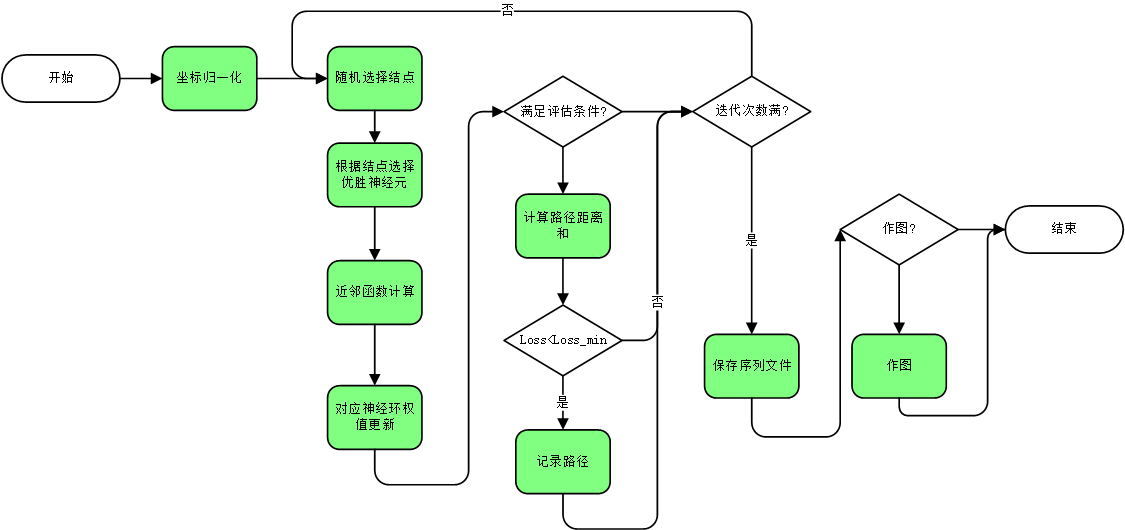
\includegraphics[width=0.95\linewidth]{fig/som-pipline}
    \end{center}
    \caption{\textbf{SOM方法流程图.} }
        \label{fig:som-pipline}
  \end{figure}


本文模型在随机选择, 优胜结点索引, 权值更新处与一般SOM模型一致, 在临近赋权时构建一维高斯函数, 对环装结点进行赋权.模型首先将节点坐标归一化, 去除偏置, 并在每次训练,获胜神经元及其近邻神经元的权值向量都会更新,经过多次反复的竞争与更新,神经网络最终学到输入数据的模式(结点的空间关系),并以神经元权值向量的形式保存下来, 体现在地图中,就是神经元的位置不断靠近城市的过程. 在解决TSP问题时, 神经元之间的竞争等价于寻找优胜神经元, 合作则等价于最优神经元更新时会带动周围其他神经元一起改变位置, 最终这会使得任意迭代步数的神经元环都能解算出一条对应的哈密顿回路, 求解的流程图如图\ref{fig:som-pipline}所示.






    
\subsection{som-TSP模型求解}

\begin{figure}[h]
    \begin{center}
        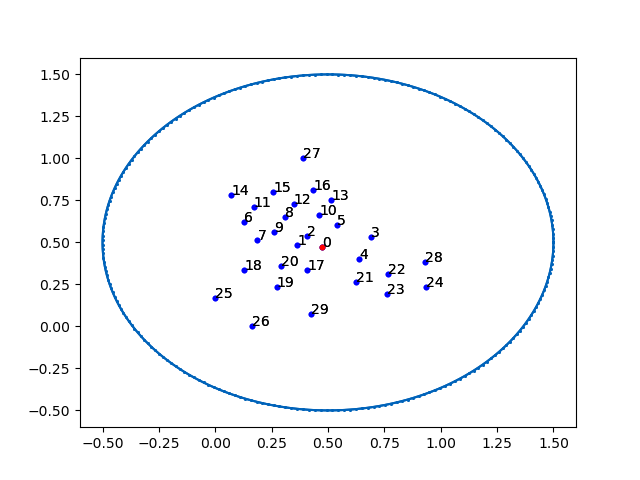
\includegraphics[width=0.55\linewidth]{fig/init}
    \end{center}
    \caption{\textbf{som-TSP模型神经环初始化.} 在求解过程中,点的坐标已经被归一化 }
        \label{fig:init}
  \end{figure}
  我们通过建立的som-TSP模型,对问题进行求解\footnote{som-TSP模型代码见支撑材料或\url{https://github.com/xdr940/som-TSP}}. 模型网络设为单层, 输出层共计210个神经元, 初始化神经环为圆形, 包裹所有点,如图\ref{fig:init}. 
模型共计迭代5000次, 每100次评估一次,评估指标为当前神经环解算出的回路总距离, 并将每次最好的结果保存. som-TSP模型求解时间在Intel I7 8700K上共计4.9s, 在第2500 次迭代中求出的最优路径, 如图\ref{fig:solution}, 长度为$L=0.1143807$, 换算后为$l = 11.43807km$. 路径为:

$p_{0}\rightarrow p_2\rightarrow p_1\rightarrow p_9\rightarrow p_7\rightarrow p_6\rightarrow p_{14}\rightarrow p_{11}\rightarrow p_{8}\rightarrow  p_{12}\rightarrow  p_{15}\rightarrow  p_{27}\rightarrow  p_{16}\rightarrow  p_{13}\rightarrow  p_{10}\rightarrow p_{5}\rightarrow p_{3}\rightarrow p_{4}\rightarrow p_{22}\rightarrow  p_{28}\rightarrow p_{24}\rightarrow p_{23}\rightarrow p_{21}\rightarrow p_{29}\rightarrow p_{26}\rightarrow p_{25}\rightarrow p_{18}\rightarrow p_{19}\rightarrow p_{20}\rightarrow p_{17}$


\begin{figure}[h]
    \begin{center}
        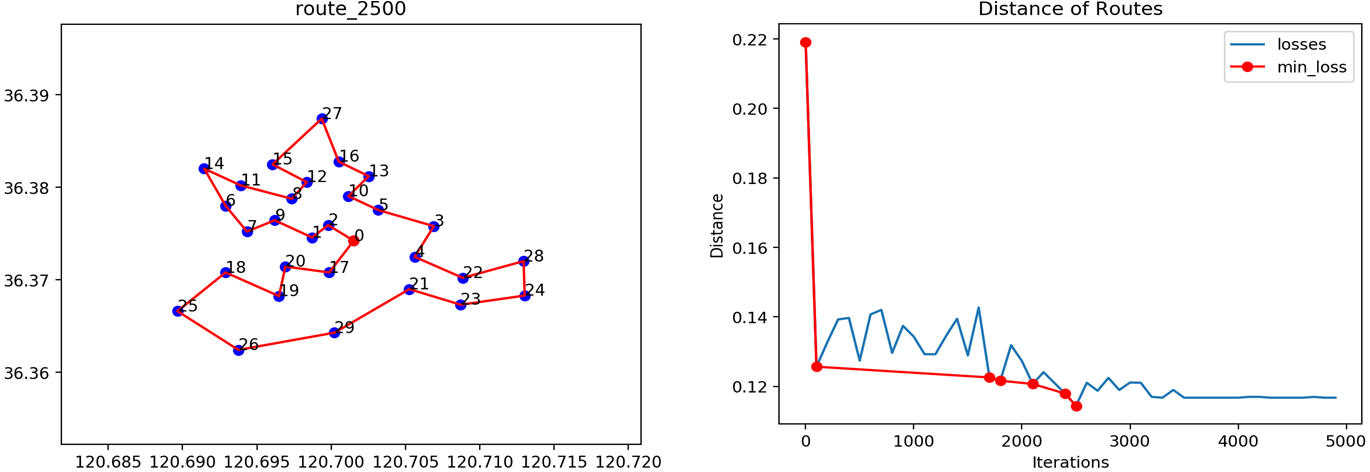
\includegraphics[width=1.0\linewidth]{fig/solution}
    \end{center}
    \caption{\textbf{最优解路径与迭代过程中路径变化.} }
        \label{fig:solution}
  \end{figure}






\begin{figure}[h]
    \begin{center}
        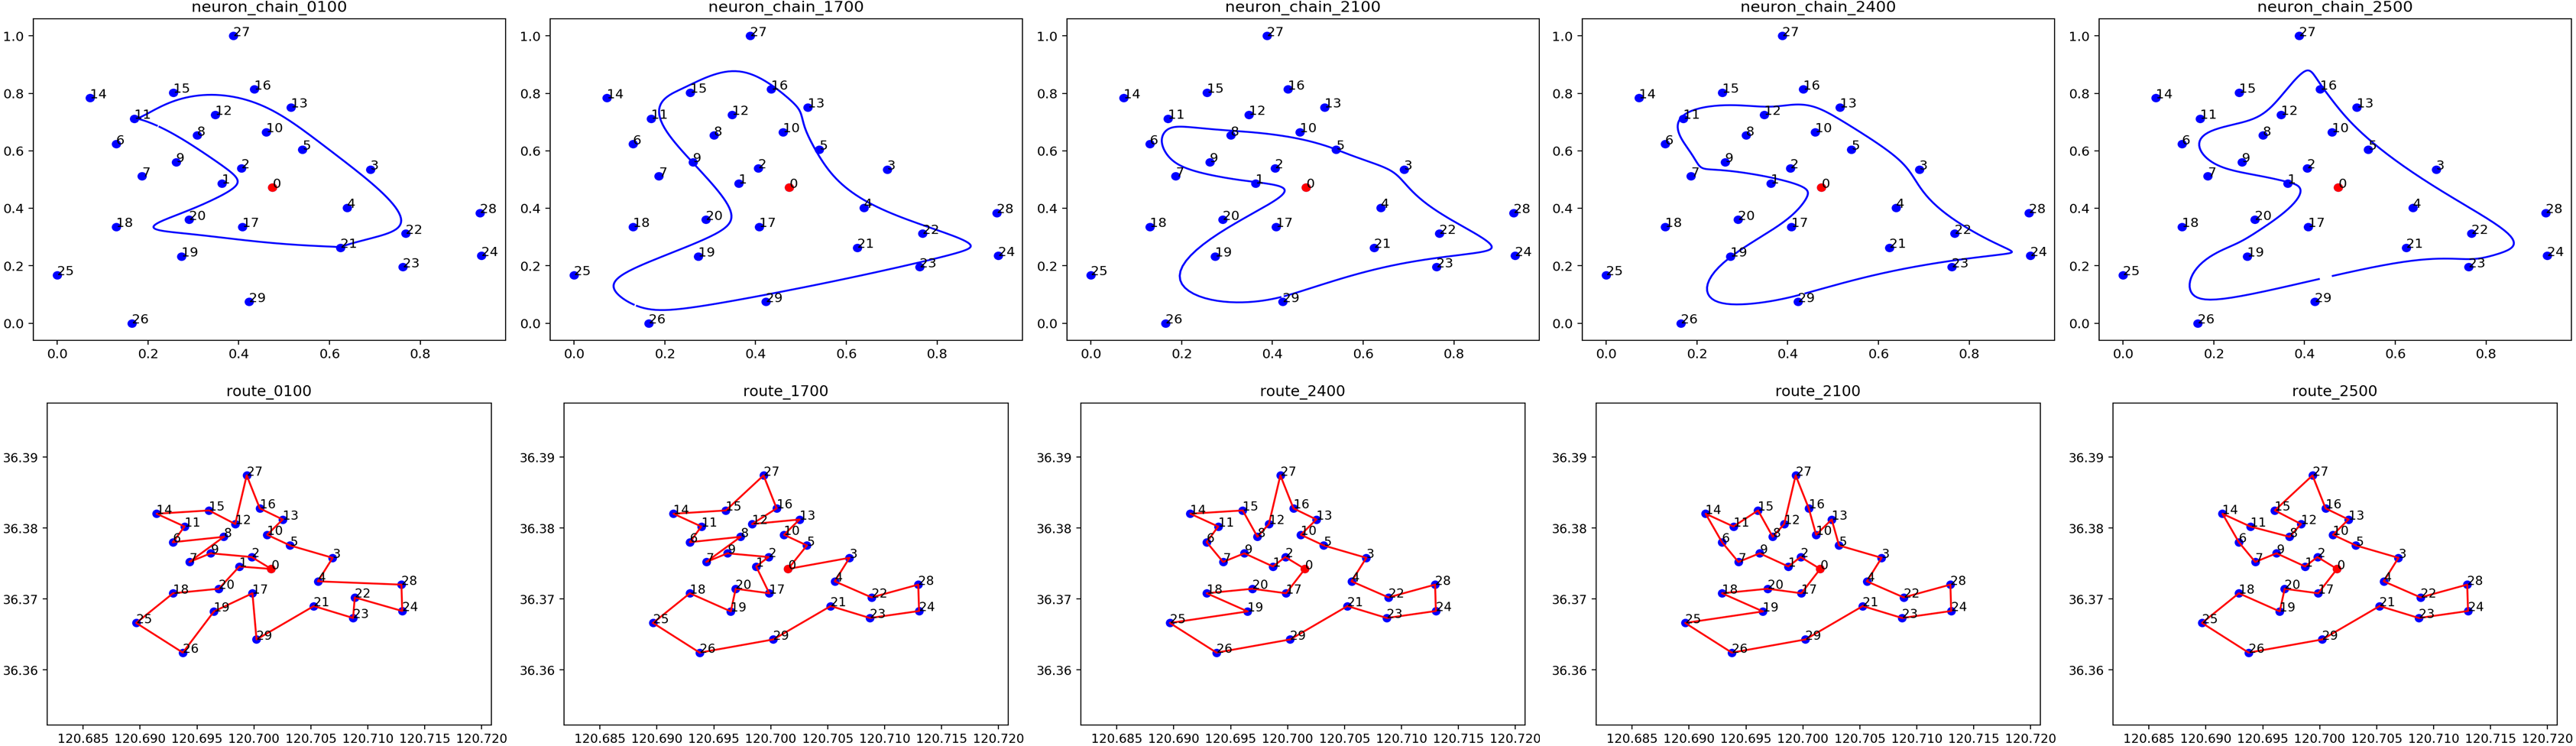
\includegraphics[width=1.0\linewidth]{fig/iteration}
    \end{center}
    \caption{\textbf{som-TSP模型求解过程.}第一行为神经元环可视化,第二行为神经元环对应的解} 
        \label{fig:iteration}
  \end{figure}
	%chapter03

\newpage
\section{问题二的模型建立与求解}
\label{sec:method2}
\subsection{问题二符号说明}

\begin{table}[h]
	\begin{center}
		\caption{问题二符号说明}
		\begin{tabular}{l|c}
			\toprule[2pt] 
			    符号 & 意义 \\ \hline
			 $i$& 传感器结点标号\\
             $T_i$&结点i充电时间\\
             $\bar{T}_i$&结点i放电时间\\
             $T$&充电系统运行一个循环的时间\\
             $T_r$&不算充电时间, 充电车行进的时间\\
			 $w_i$&结点i电量消耗功率\\
			 $f$&结点电池电量底线\\
			 $c_i$&结点电池电量\\
			 $v$&充电车行进速度\\
             $r$&充电车充电功率\\
			 $N$&充电结点个数\\
			
			\toprule[2pt] 
		\end{tabular}
		
		\label{tab:distribution}
		\vspace{-0.4cm}
	\end{center}
\end{table}


\subsection{问题二的模型建立与求解}
根据问题一的求解, 已经得到环路, 根据问题二题干描述, 我们可以假设到整个系统稳定时, 充电车应在该环路循环跑动, 且运行一圈时间固定不变. 在系统运行时, 电池可能的最小容量即为耗电量最大的结点, 而对于充电速率统一为$r$, 耗电量最大的结点充电时间最长的结点. 又因为所有节点的电池容量统一, 故电池容量最小应为:

\begin{eqnarray}
    c_{min} = \mathop{Max} T_i \cdot r + f
    \label{eq:cmin}
\end{eqnarray}

其中$c_{min}$为电池最小容量, $T_i$为结点$p_i$的充电时间, $r$为充电功率, $f$为电池最低电量.

上式中, 充电时间$T_i$为变量, 故可建立充电时间模型, 求出每个结点最小充电时间, 则问题解决.

设数据中心为$p_0$点, 电动车跑完一轮时间为$T$, 每个结点充的电量为$c_i$, 充电车对$p_i$点充电时间为$T_i$, 则$p_i$点每个循环电量消耗时间为$\bar{T}_i = T-T_i$, 放电功率为$w_i$,故消耗电量为$w_i(T-T_i)$, 则可列方程:

\begin{eqnarray}
c_i = w_i \bar{T_i} = w_i(T-T_i)\leq rT_i 
\end{eqnarray}

将不等式移项, 将$T_i$分离出, 则有

\begin{eqnarray}
\nonumber
\quad &\frac{w_iT}{r+w_i} \leq T_i&\\
\nonumber
\quad &\frac{w_i}{r+w_i} T_{r} + \frac{w_i}{r+w_i} \sum\limits_{j\neq i } T_j - T_i \leq 0,~~ i =0,1,2,\dots N&
\end{eqnarray}
这里, $T_r$为充电车不算充电, 行走的时间; $N$为所有结点个数
令$\frac{w_i}{r+w_i} = a_i, \textbf{a} = [a_1, a_2, \dots a_N], ~\textbf{T} = [T_0,\dots T_i \dots T_N]$
则上式可化为
\begin{equation}       %开始数学环境
    \left[                 %左括号
      \begin{array}{cccc}   %该矩阵一共3列,每一列都居中放置
        a_1-1 & a_2 & \dots& a_N \\  %第一行元素
        a_1 & a_2 -1 & \dots& a_N \\  %第二行元素
        &&\dots&\\
        a_1&a_2&\dots&a_N-1\\
      \end{array}
    \right]                 %右括号
    \left[
        \begin{array}{cccc}
         T_0\\
         T_1\\
         ... \\
         T_{N}
        \end{array}
    \right ]
    +
    \left[
    \begin{array}{cccc}
     a_{1}\\
     a_{2}\\
     ... \\
     a_{N}
    \end{array}
    \right ]
    T_r \leq \textbf{0}_N
    \end{equation}

  

    \begin{equation}     
        \left\{
            \left[                 
                \begin{array}{cccc}   
                1 & 0 & \dots& 0 \\  
                0 & 1  & \dots& 0 \\ 
                &&\dots&\\
                0&0&\dots&1\\
                \end{array}
            \right] 
            -
            \left[                 
            \begin{array}{cccc}   
                a_1 & a_2 & \dots& a_n \\ 
                a_1 & a_2  & \dots& a_n \\  
                &&\dots&\\
                a_1&a_2&\dots&a_n\\
            \end{array}
            \right]    
        \right\}   
        \left[
            \begin{array}{cccc}
             T_0\\
             T_1\\
             ... \\
             T_{n}
            \end{array}
        \right ]
        \geq
        \left[
            \begin{array}{cccc}
            a_{1}\\
            a_{2}\\
            ... \\
            a_{n}
            \end{array}
        \right ]
        T_r 
        \end{equation}

其中, $\textbf{0}_N$为N维零向量. 上式可化为:
\begin{eqnarray}
  (\textbf{I}- \textbf{1}^T\textbf{a} )\textbf{T} \geq \textbf{a} T_r
\end{eqnarray}
所以
\begin{eqnarray}
  \textbf{T} \geq   (\textbf{I}- \textbf{1}_N^T\textbf{a} )^{-1}\textbf{a} T_r
\end{eqnarray}
因为$T_i \geq 0$所以有:
\begin{eqnarray}
    \mathop{Max}T_i = \| (\textbf{I}- \textbf{1}_N^T\textbf{a} )^{-1}\textbf{a} T_r\|_{\infty}
\end{eqnarray}
这里$\|\cdot\|_\infty$为无穷范数, 用来求分量中最大项; $\textbf{1}_N$为N维全1向量. 再将$ T_r = l/v$ 带入,联合方程\ref{eq:cmin} 得到

\begin{eqnarray}
    c_{min} =r \| (\textbf{I}- \textbf{1}_N^T\textbf{a} )^{-1}\textbf{a} \frac{l}{v}\|_{\infty} +f
\end{eqnarray}

综上, 求得整个充电系统中电池最小容量为$ c_{min} =r \| (\textbf{I}- \textbf{1}^T\textbf{a} )^{-1}\textbf{a} \frac{l}{v}\|_{\infty} +f $. 另外, 考虑数据中心结点处充电车停留时间为0, 计算时要将$T_0 = 0$带入计算.


%其中, $T = T_{charge} + T_{run}$, $T_{charge} = \sum \limits_{i} T_i  $. $T_{run} = l/v $







	\section{问题三的模型建立与求解}



\subsection{多重旅行商问题}
问题三为多旅行商问题即mTSP(Multiple Traveling Salesman Problem), 与TSP类似, 该类问题同属于NPC问题. 文献\cite{surveymtsp}中对此问题进行了详细的分析, 多重旅行商问题为TSP的衍生问题, 其也可以分为多个变种, 比如根据仓库depots点的个数或者旅行商数量而区分\cite{mtsp-genetic}, 通过进化算法求解mTSP比较常见\cite{AdlemanTSP,mtsp-genetic}, 本文我们通过SOM模型对其进行求解.



\subsection{SOM模型求解多重旅行商问题}

我们将SOM模型推广, 构建了可以解决m个旅行商下n个仓库点的问题的模型som-mTSP\footnote{som-mTSP代码见支撑材料或\url{https://github.com/xdr940/som-mTSP}}. 在本文中, 考虑一个仓库点,4个旅行商的问题. 找到四条环路$G_A, G_B,G_C,G_D$, 使得四条环路的总距离最小$\sum\limits_k l_k$, 且有$A \cap B \cap C \cap D = {p_0}$, 这里$A,B,C,D$分别为四条路径的点集合.

\noindent{\textbf{问题初始化}}\\

在问题2的模型建立中, 我们参考文献\cite{isom2008}初始化神经元环形状,并迭代. 本问题中为四个旅行商的mTSP, 则需要四个神经元环, 我们这里定义为$R_A,R_B,R_C,R_D$. 同问题一(Sec.\ref{sec:method1})一样, 神经元环对应的权值向量对应着2维空间坐标, 可视化如图\ref{fig:init2}
\begin{figure}[h]
    \begin{center}
        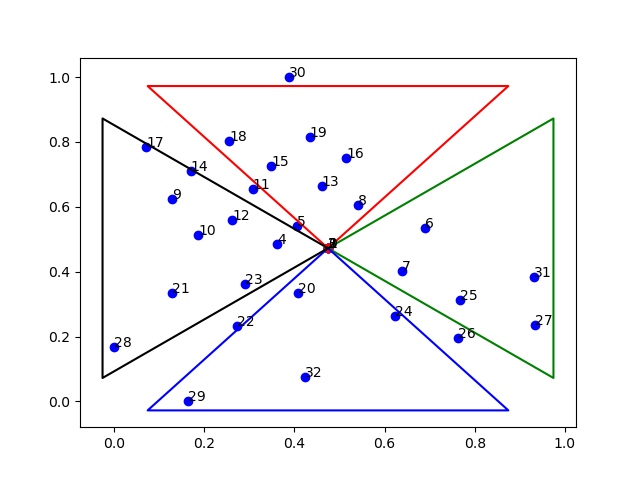
\includegraphics[width=0.55\linewidth]{fig/init2}
    \end{center}
    \caption{\textbf{som-mTSP模型中四条神经环初始化.} 在求解过程中,点的坐标已经被归一化 }
        \label{fig:init2}
  \end{figure}

\noindent{\textbf{优胜选择(Winner selection)}}\\

由于神经环在本问题中有多个, 故将优胜选择函数重新构建, 设计为两个, 一个求解对于$X_i$结点最近的神经环索引, 另一个求解在此神经环中最近神经元的索引.
\begin{eqnarray}
    k = \mathop{argmin}\limits_{k}\{ |X_i-W^k_j(n)|\beta(k) \}\\
   \nonumber
    j = \mathop{argmin}\limits_{j}\{ |X_i-W^k_j(n)|\beta(k) \} \\
    \nonumber
    \beta(k) = 1+\frac{l_k - l_{avg}}{l_{avg}},~~ k \in \{A,B,C,D\}
\end{eqnarray}

其中$l_k$是充电车在环路$G_k$行进一圈的距离,$l_{avg}$是充电车行进的平均距离, $|\cdot|$表示欧几里得距离. 此函数包括两个部分:$R_k$上的节点$W^k_j$与城市节点$X_i$之间的欧式距离,以及四个环路各自距离与平均距离的偏差$\beta(k)$. 在考虑$G_k$时,如果$l_k \leq l_{avg}$,则$R_k$上的节点的电位小于相应的欧几里得距离;因此, 将选择环$R_k$上的节点并移向所显示城市的机会更高 否则,如果$l_k \geq l_{avg}$,则选择环$R_k$上的节点的机会将减少, 该偏差可被视为需要调整每个环以获得相似距离的 minmax 约束\cite{som-mtsp2}.


\noindent{\textbf{近邻计算}}\\

我们对多个神经元环使用统一的学习率$\alpha$和半径衰减函数$\sigma$, 这里函数设定同章节(Sec.\ref{sec:preliminary})一致.

\begin{eqnarray}
    \quad & T(j,i,n) = e^{ - \frac{S^2(i,j)}{2\sigma^2(n)}}&\\
    \quad &\sigma(n) = \sigma_0e^{- n\verb|/|\tau}&
  \end{eqnarray}

\noindent{\textbf{适应(Adaption)}}\\

对于每个神经环$R_k$, 都有相同的权值更新函数:
\begin{eqnarray}
    \quad &W_j^k(n+1) =  W_j^k(n)+\alpha(n) T \cdot |X_i - W_j^k(n)|, k \in{A,B,C,D}&\\
    \nonumber
    \quad & \alpha(n) = \alpha_0e^{- n  \verb|/| \tau}&
\end{eqnarray}
这里$\alpha_0$为初始化学习率, $\tau$为衰减率, 一般设为0.99
\subsection{求解路径}
我们通过建立的som-mTSP模型, 对问题进行求解. 并预设神经元个数为每个环100个, 迭代5000次, 没100次对模型进行一次评估, 评估指标为四条环路的总长度, 并将每次最好的结果保存.

som-mTSP模型求解时间在Intel I7 8700K上共计5.6s, 求解过程以及结果可视化\footnote{支撑材料中有gif动图}见图\ref{fig:mtsp-solution}. 我们改进的模型可求解m个旅行商,n个仓库点的情况,对于问题3中$m=4, n=1$的条件, 我们将数据预处理,添加三个与$p_0$坐标相同的点, 定义为$p_1,p_2,p_3$\footnote{后文中所有点包括图示的应该减3}.
最终, 模型在迭代2200次时找到最优解,四条路径分别是:
\begin{eqnarray}
    \nonumber
   A: p_0 \rightarrow p_5 \rightarrow p_{13} \rightarrow p_{16} \rightarrow p_{27} \rightarrow p_{15} \rightarrow p_{12} \rightarrow p_{10}, l_A=0.0317137\\
    \nonumber
  B:  p_0 \rightarrow p_{4} \rightarrow p_{21} \rightarrow p_{22} \rightarrow p_{23} \rightarrow p_{24} \rightarrow p_{28} \rightarrow p_{3}, l_B=0.0355413\\
    \nonumber
   C: p_{0} \rightarrow p_{20} \rightarrow p_{18} \rightarrow p_{25} \rightarrow p_{26} \rightarrow p_{29} \rightarrow p_{19} \rightarrow p_{17}, l_B=0.0408157\\
    \nonumber
    D: p_{0}\rightarrow p_{1}\rightarrow p_{9}  \rightarrow p_{7} \rightarrow p_{6} \rightarrow p_{14} \rightarrow p_{11} \rightarrow p_{8} \rightarrow p_{2}, l_D=0.028521
\end{eqnarray}
距离分别为
\begin{eqnarray}
    &l = l_A+l_B+l_C+l_D = 0.136592&
\end{eqnarray}
$l$根据模型假设, 换算为$l= 13.6592$km
%并添加约束, 即每个神经环$R_k$求解出的环路$G_k$必须包含一个仓库点.. 

\begin{figure}[h]
    \begin{center}
        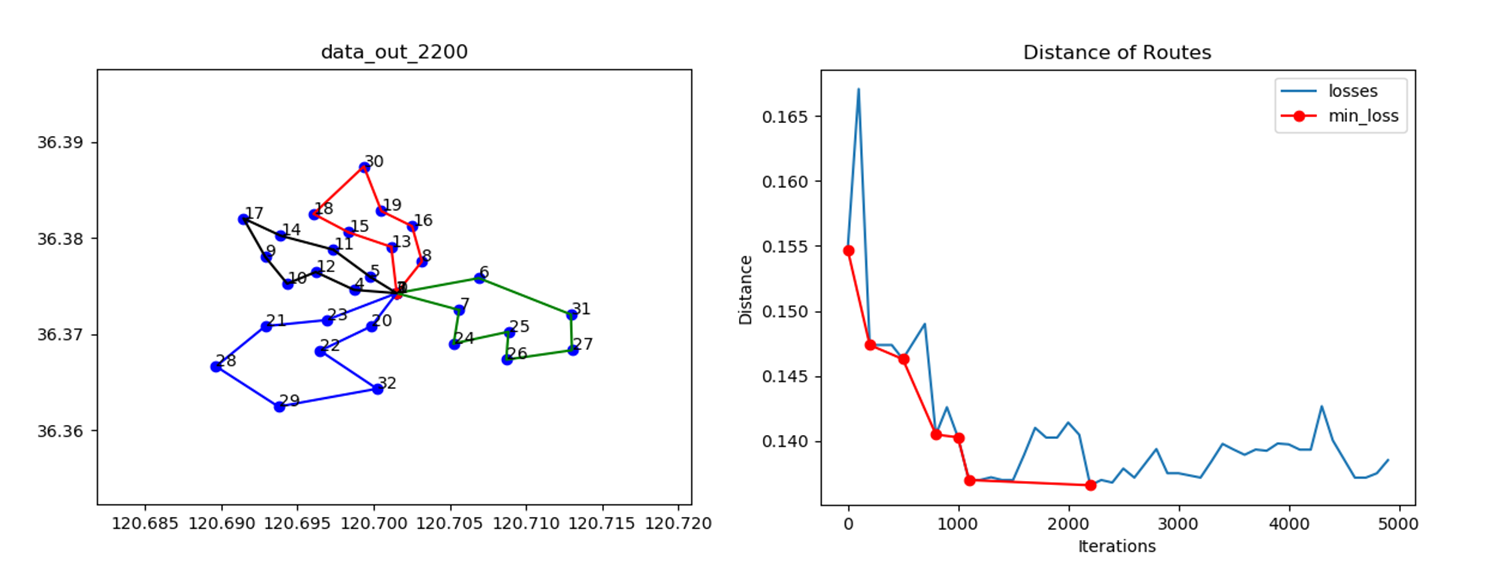
\includegraphics[width=0.95\linewidth]{fig/solution2}
    \end{center}
    \caption{\textbf{som-mTSP最优解路径.} }
        \label{fig:mtsp-solution}
  \end{figure}


\begin{figure}[h]
    \begin{center}
        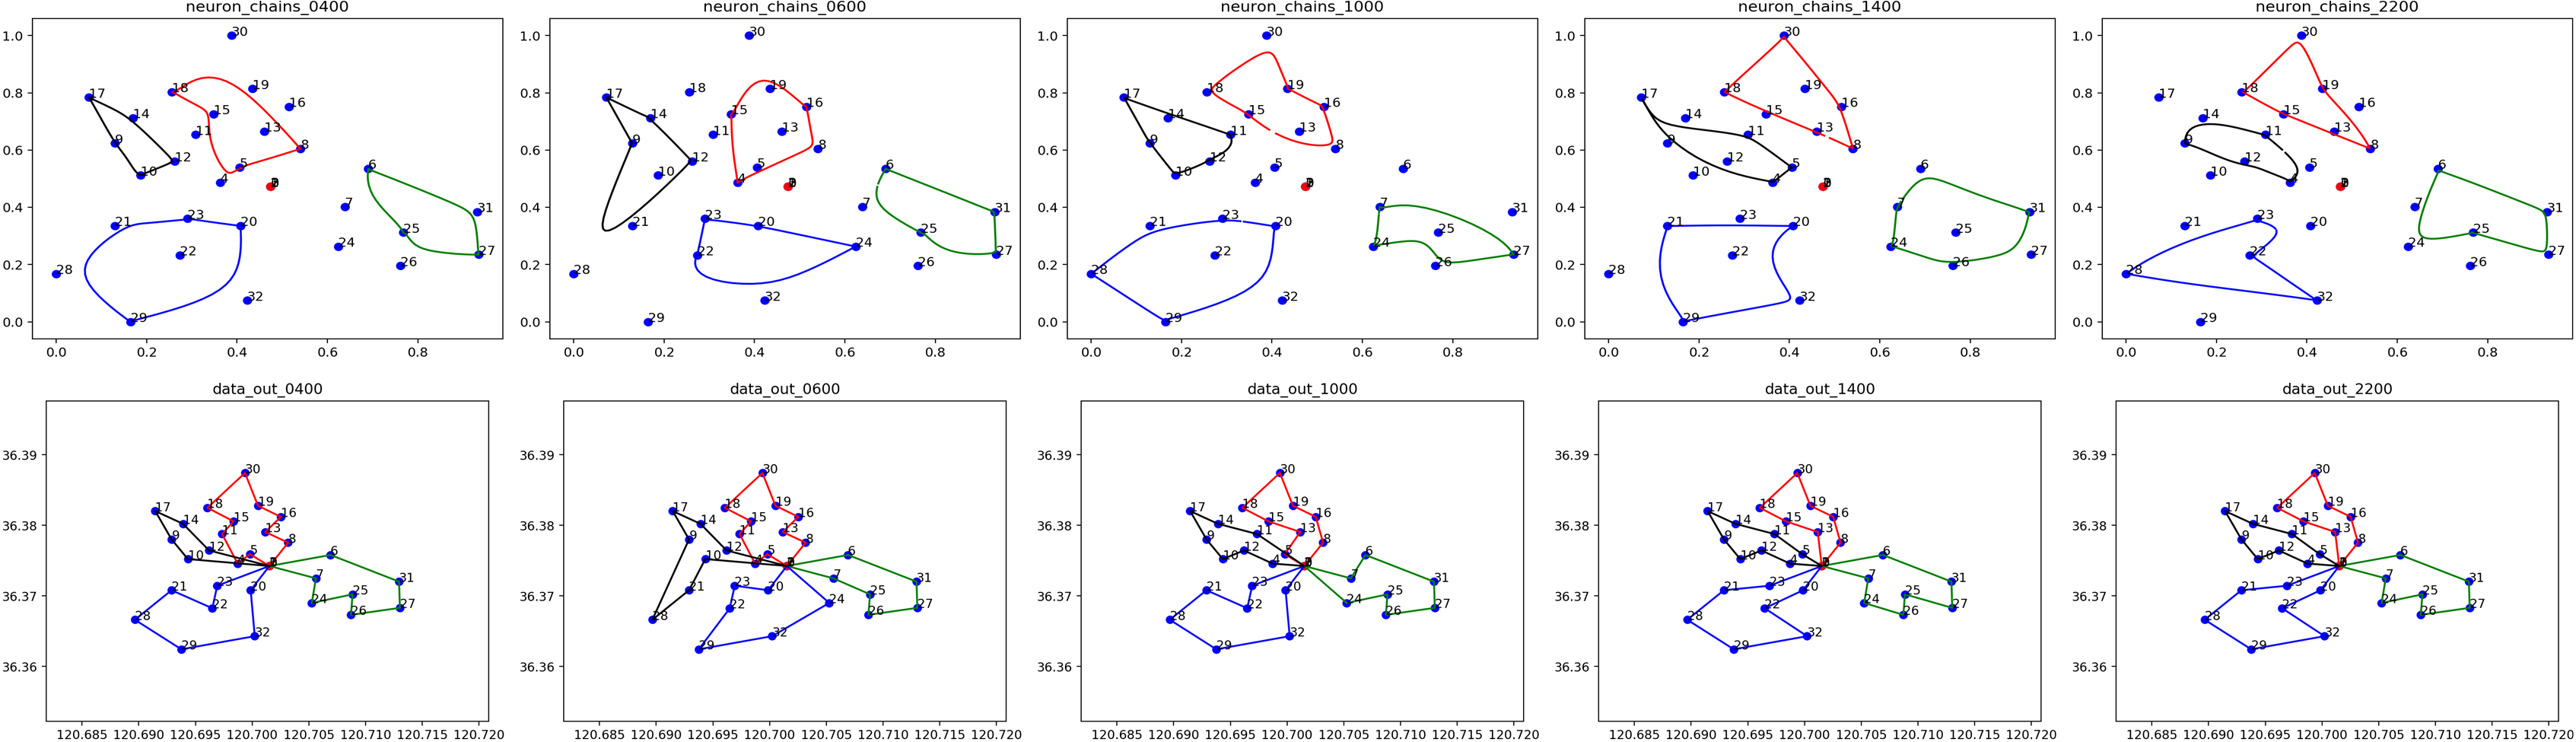
\includegraphics[width=1.0\linewidth]{fig/iteration2}
    \end{center}
    \caption{\textbf{som-mTSP求解过程.}第一行为神经元环可视化, 第二行为神经环对应的解} 
        \label{fig:iteration}
  \end{figure}

\subsection{多移动充电器下的电池最小容量求解}

在四条路径已经规划出的前提下, 每条子路径中电池最小容量与问题2求解类似(Sec.\ref{sec:method2}), 故我们使用问题二中的优化模型对本问题进行求解. 通过最小充电时间模型我们求出每个结点允许的最小充电时间, 通过最小充电时间可以求得每个子环路的最小电池容量, 而整个系统的最小电池容量即为四条环路中允许电池容量的最大值.
假设四条路径包含的点集分别为$A,B,C,D$, 则有:


\begin{eqnarray}
    c^k_{min} =r \| (\textbf{I}_k- \textbf{1}^T\textbf{a}^k )^{-1}\textbf{a}^k \frac{l^k}{v}\|_{\infty} +f ,~~k \in \{A,B,C,D\}
\end{eqnarray}
这里$\textbf{a} = [a_1, a_2, \dots a_n],~ a_i = \frac{w_i}{r+w_i}$,$|\cdot|_\infty$ 为无穷范数, $l^k$根据som-mTSP模型已经以分别求出, 故整个系统的电池最小容量为:
\begin{eqnarray}
    c_{min} = \mathop{Max}\{c^A,c^B, c^C,c^D\}
\end{eqnarray}

	\section{模型推广与比较}

%SOM模型在小型数据集上效果与常规软计算(Soft-Computing)方法相比, 优势并不明显, 为了验证模型具有更好的一般性, 可以适应较大的数据集, 我们对模型进行了推广与比较.
TSP及其相关问题的算法一般通过TSPLIB平台进行评估,TSPLIB\cite{Reinelt1991TSPLIB}是旅行商问题以及相关问题构建的数据集, 包括对称旅行商(CTSP,TSP)问题, 哈密顿回路问题(HCP)以及非对称旅行商问题(ASTP)等. TSP问题中最通常的评估方法为"偏离最优率$\mu$", 即算法得到路径长度超出TSPLIB公布最优结果的百分比, $\mu$越小表明算法得到解的质量越高.
部分工作对TSP中的不同方法已经进行了充足研究和大量的对比实验. 

文献\cite{som-mtsp2}提出了引入局部渗透机制的ISOM方法, 并对同属于SOM类算法的NIES\cite{N2003A}, SETSP\cite{SETSP}, Budinich 和ESOM\cite{ESOM}之间的横向对比, 结果如\ref{fig:som-cp}所示, 其试验结果显示SOM变种方法运行时间基本上是都是按照城市数量的二次关系递增的, 保持了SOM算法具有较低计算复杂度的优良特点.
\begin{figure}[h]
    \begin{center}
        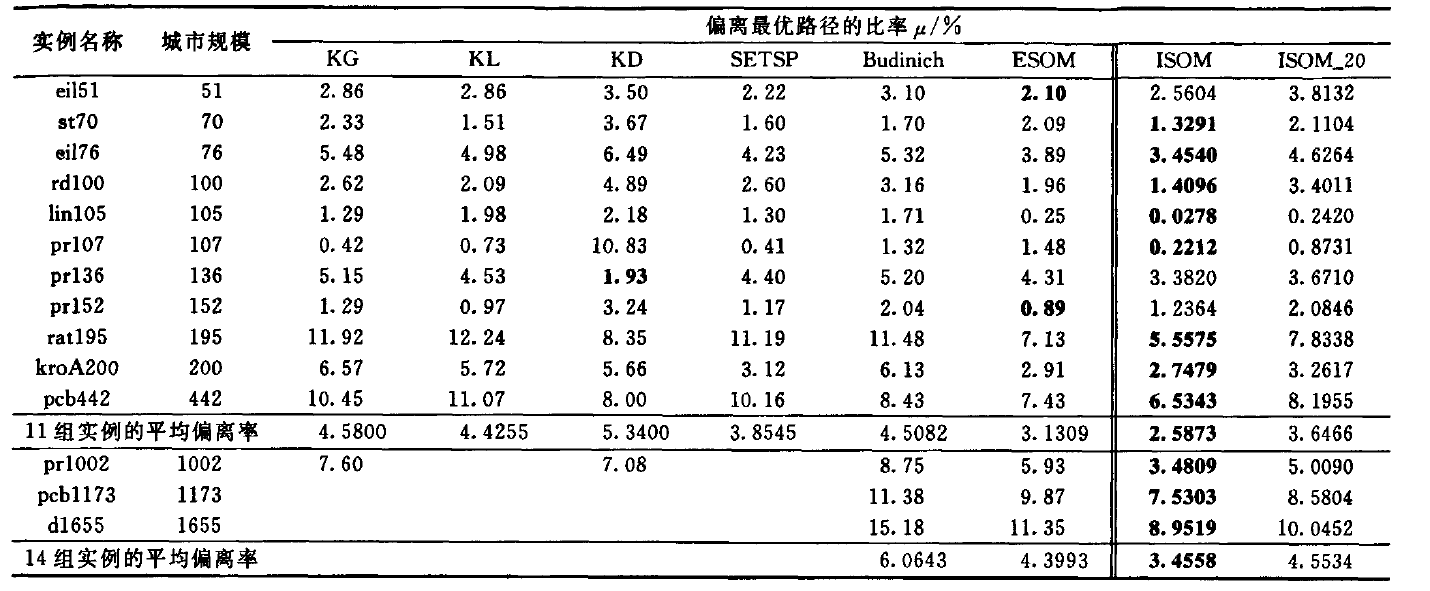
\includegraphics[width=0.85\linewidth]{fig/som-cp}
    \end{center}
    \caption{\textbf{几种SOM方法在TSPLIB上的结果.}实例尾标数字代表图中点数 }
        \label{fig:som-cp}
\end{figure}


文献\cite{2007Kohonen}对SOM类方法和其他进化算法(包括遗传, 蚁群以及退火等常见进化算法)进行了横向的的比较,图\ref{fig:som-cp2}可以在求解时间一栏内明显看到SOM类算法的低复杂度特性, 虽然其在点数较少的情况下容易陷入局部最优, 解的质量不如传统的进化算法, 但在针对大点数数据集中有着明显的效率优势.
\begin{figure}[h]
    \begin{center}
        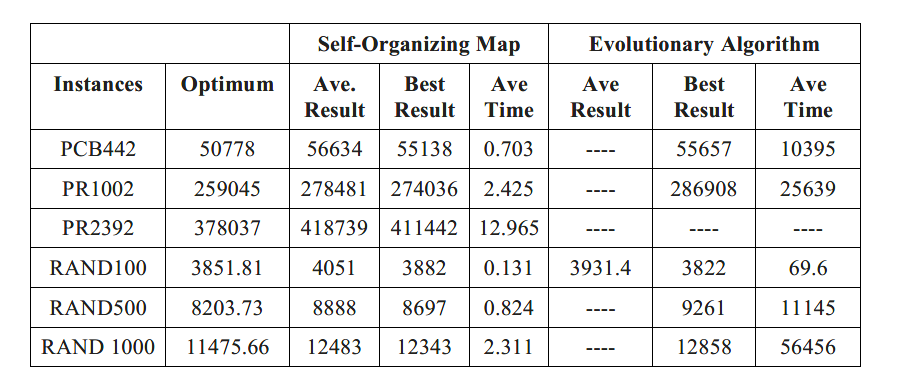
\includegraphics[width=0.65\linewidth]{fig/som-cp2}
    \end{center}
    \caption{\textbf{SOM方法与进化算法在TSPLIB上的结果.}实例尾标数字代表图中点数 }
        \label{fig:som-cp2}
\end{figure}

%文献\cite{som-mtsp2}还对SOM方法在多旅行商问题上进行了消融试验,%, 这里将主要在SOM方法与其他方法在TSP问题中的比较和类SOM方法在TSP中的比较做阐述.










	\section{总结讨论}

针对问题一,本文引入som-TSP模型(Sec.\ref{sec:method1}), 对充电车进行路径规划, 旨在寻找30个传感器结点组成图的哈密顿回路, 并求出结果为$L = 11.43807$ km;
针对问题二, 本文建立优化模型, 通过最小化每个结点的充电时间建模求解而得到电池电量的允许最低值的解析解;
针对问题三, 本文将SOM模型根据文献\cite{som-mtsp}进行修改, 建立som-mTSP模型, 并编程实现求解, 得到四条路径和为$l_{A+B+D+C} = 13.6592$km, 另外, 基于求得的四条最优路径, 根据问题二的优化模型, 我们通过同样方法求解得到每条路径的最低电池容量, 从而求解得到整个系统允许的最低电池容量的解析解.

由于TSP及其相关问题皆为NP-完全问题, 本文在解决TSP以及mTSP问题上, 主要借助基于人工神经网络SOM模型及其变体的"软计算"方法, 通过逼近的策略而解得最优解, 模型在一维环形SOM网络在TSP问题求解具有相当的合理性. 就解决问题方法而言, 基于进化算法的求解方法在小规模数据上表现良好, 但在大点数情况下无论其求解时间还是精度都有着比较明显的问题, 而神经网络方法的优缺点相比较前者又恰好相反. 随着结合二者优缺点的方法相继提出, 此类问题也许会渐渐得到更好的解决.

从理论和实践两个方面来看,多重旅行商问题(mTSP)都是一个重要的问题. 首先, 此类问题概括了旅行商问题(TSP), 可以进行研究以从理论角度更好地理解TSP. 另一方面, 通过合并诸如容量, 距离和时间窗口限制之类的附加侧面限制, 可以轻松地将其扩展到更具一般性的车辆路径问题(VRP). 对mTSP的深入研究无论泛化到更一般的问题还是具象为更特殊的问题, 在实际生活中都有着大量的应用背景, 研究价值巨大.

%本文涉及代码与模型, 皆为队员原创





	%参考文献
	\kaishu
	\bibliographystyle{unsrt}
	\addcontentsline{toc}{section}{参考文献} %向目录中添加条目,以章/section的名义
	\bibliography{ref.bib}
%\clearpage
\begin{appendices}

	\section{计划和分工与团队构成}



\end{appendices}

	\label{lastpage}%%%%显示总页数
\end{document}